% -*- latex -*-
%%%%%%%%%%%%%%%%%%%%%%%%%%%%%%%%%%%%%%%%%%%%%%%%%%%%%%%%%%%%%%%%
%%%%%%%%%%%%%%%%%%%%%%%%%%%%%%%%%%%%%%%%%%%%%%%%%%%%%%%%%%%%%%%%
%%%%
%%%% This text file is part of the source of
%%%% `Parallel Programming in MPI and OpenMP'
%%%% by Victor Eijkhout, copyright 2012-2025
%%%%
%%%% cuda.tex : cuda
%%%%
%%%%%%%%%%%%%%%%%%%%%%%%%%%%%%%%%%%%%%%%%%%%%%%%%%%%%%%%%%%%%%%%
%%%%%%%%%%%%%%%%%%%%%%%%%%%%%%%%%%%%%%%%%%%%%%%%%%%%%%%%%%%%%%%%

\Level 0 {Host and device}

Analogous to how OpenMP marked certain regions as parallel,
a \ac{CUDA} program marks certain function calls as
executable on a device.
\begin{itemize}
\item Host: the CPU where the execution starts
\item Device: one of possibly several attached \acp{GPU}.
\end{itemize}
Device code is recognizable by a keyword prefix,
either \indexcudashow{__global__} or \indexcudashow{__device__}.
The \indexcudashow{__host__} keyword marks host code, but that's the default.

\begin{lstlisting}
__global__ void some_cuda_function( /* parameters */ );
\end{lstlisting}
Device code needs have type \lstinline{void}:
return results have to be passed explicitly through memory.

\Level 1 {Hello world}

A device function that prints hello:
\cudaverbatimsnippet{cuhellodef}
And the main program launches this kernel on a grid of one block of size~1.
\cudaverbatimsnippet{cuhellouse}
We need the \indexcudashow{cudaDeviceSynchronize} function so that the host waits
until all device actions are completed.
\begin{figure}[ht]
  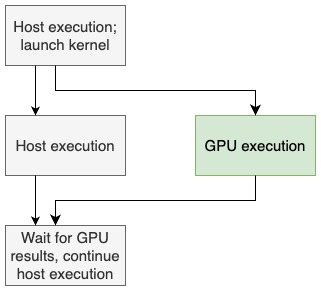
\includegraphics{hostgpuoverlap}
  \caption{Host and device activity}
  \label{fig:hostgpuoverlap}
\end{figure}
Normally, host and device actions can take place concurrently;
see figure~\ref{fig:hostgpuoverlap}.

The `triple chevron' syntax indicates how many block, and how many threads per block,
are used to launch the kernel.
You can put a 2D or 3D structure on the blocks by using the \indexcudashow{dim3}
coordinate structure:
\cudaverbatimsnippet{cuhello3use}
The coordinate of the block and the thread within the block can now be
found through the \indexcudashow{blockIdx} and \indexcudashow{threadIdx}
coordinate structures.

While the number of blocks can be large, the number of threads is limited.
The $x,y$ sides of the block cannot exceed~$1024$, and the $z$~side
can not exceed~$64$; the total size of the block is limited to~$1024$.

\Level 1 {Thread indexing}

We need a way of identifying which CUDA thread executes a kernel.
Each kernel execution can query the (globally defined) variables
\indexcudadef{blockIdx} and \indexcudadef{threadIdx}.

It is possible to launch a kernel on more threads than
there are data points. In that case, your code could include
\begin{lstlisting}
int global_thread_id = blockIdx.x * blockDim.x + threadIdx.x; // or 2d, 3d variant
if ( global_thread_id > datasize ) return;
\end{lstlisting}

\Level 1 {Data transfer}

The host and device have separate memory, so you may need to
synchronize host data to the device.

\Level 2 {Explicit copy}

One strategy is allocate data separately for host and device.

Device memory is allocated with \indexcudashow{cudaMalloc}.
While the resulting pointer is visible to the host code,
the actual memory is on the device and you need to transfer data explicitly
between host and device with \indexcudadef{cudaMemcpy}.
This transfer can be between host and device in either direction,
or between two devices.

\begin{lstlisting}
cudaMemCpy( dest_ptr, orig_ptr, byte_size, direction );
// direction:
cudaMemcpyHostToDevice
cudaMemcpyDeviceToHost
cudaMemcpyDeviceToDevice
\end{lstlisting}

Example:
\cudaverbatimsnippet{cuhostdevalloc}

The data is then copied to the \ac{GPU}:
\cudaverbatimsnippet{cudatacopyin}
and after the kernel execution resulting data is copied back:
\cudaverbatimsnippet{cudatacopyout}

\Level 2 {Managed memory}

You can also allocate memory in a more abstract way:
`managed memory' can be written on the host,
but accessed from the device.
The actual mechanism that moves data back and forth
is based on \indexterm{paging}.
\cudaverbatimsnippet{cumanagedalloc}
